\chapter{Stochastic Chemcal Kinetics} \label{ch:cme}

\section{Stochasticity in Cell Dynamics}

The formalism and example systems in the preceed chapters tacitly make
the assumption that there are so many molecules in the system of
interest that small fluctuations in the quantities, positions,
energies, etc. of these molecules do not contribute significantly to
the dynamics of the system. However, when we compare the behaviors of
individual isogenic cells, we see substantial variation in their
behaviors. For example, starting from isogenic and synchronized {\em
  E. coli} cells, the time between cell divisions is observed to be
highly variable, ranging from 30 to 60 minutes [CHECK THIS] at a given
temperature \cite{plank-harvey}. As another example, in bacterial
chemotaxis, cells respond to the addition of uniform attractant by
swimming smoothly, but relax back into tumbling at random times
\cite{spudich-koshland}. And as a third example, {\em E. coli} have
been see to switch to and from presenting type I {\em fimbriae} at
random time \cite{galley-fim}.

Two types of randomness have been proposed in the literature
\cite{swain-in-ex}: {\em Intrinsic} and {\em Extrinsic}. The former
has to do with randomness that is part of a system of interest and
that may be due to the fact that a given transcription factor may be
present in integral quantities: 0, 1, 2, etc. In this case, one has
to, for example, rethink what chemical equilibrium means: it may be
that on average the number of molecules of each type is fixed, but
reactions are still occuring and variations in the amounts of them can
be significant. The latter has to do with ...

% Examples from Elowitz, Van Oudenaarden, Arkin, etc.

\section{Foundations of Stochastic Chemical Reactions}

% assumptions
The common assumption in modeling stochastic chemical systems is that
the system is {\em well-mixed}. Mathematically, this means:
%
\begin{enumerate}
\item \label{wm1} The probability that a given pair of molecules
  reacts in the next $dt$ seconds is independent of time;
\item \label{wm2} A given molecule is equally likely to interact with
  every other molecule in the system.
\end{enumerate}
%
Physically, the assumptions \ref{wm1} and \ref{wm2} can arise if the
rate of diffusion is much higher than the rate of reaction, so that
the molecules are essentially uniformly distributed over the
containing volume. In this case, every instant of time is essentially
the same in terms of where the molecules are, and thus how the
molecules arrived there is irrelevant. 

Consider a vessel containing two molecules, $A$ and $B$, that react to
form a product molecule $C$ according to
%
$$
A+B \xrightharpoon[\text{}]{\text{$k$}} C
$$
%
where $k dt$ is defined to be {\em the probability that molecules $A$
  and $B$ react to form a $C$ in the time interval $[t,t+dt)$.}
Define by $f(t)$ the probability density function for when in time the
reaction occurs when the system is started at time $0$. Then
%
$$
F(t) = \int_0^t f(\tau) d \tau
$$
%
is the probability that the reaction occurs in time $[0,t]$. Suppose
the reaction has not occured by time $t$. Because the system is
well-mixed, we require that the probability density function $g(t)$
for when the reaction occur later, given that it has not occured at
time $t$, is distributed identically to $f(t)$, except shifted in
time. We can use this notion to determine an exact expression for
$f(t)$.

First, put
%
$$
G(t) = 1 - F(t)
$$
%
to be the cumulative distribution for the event that the reaction
occurs after time $t$.  Define $T$ be the random variable defining
when the reaction occurs, so that $G(t) = P[T>t]$. Then the well-mixed
assumption, essentially the same as the Markov assumption that future
events only depend on the current state of the process, requires that
%
$$
P[T>t+\tau | T > \tau] = P [T>\tau] .
$$
%
Using Bayes rule, we have
%
$$
P[T > t+\tau] = P[T>t] P[T>\tau], 
$$
%
which amounts to
%
$$
G(t+\tau) = G(t)G(\tau). 
$$
%
The only reasonable (integrable, analytic) function that satisfies the
above equation is the exponential, so that $G(t) = e^{-\alpha t}$ for
some $\alpha > 0$ (See Exercise~\ref{ex:exponential}). Since $F(t) = 1
- G(t)$ we have that
%
$$
F(t) = 1 - e^{-\alpha t}
$$
%
and $f(t) = \frac{d}{dt} F(t) = \alpha e^{-\alpha t}$. To determine
what $\alpha$ is, note that $F(dt) = k dt$ so that $f(0) = \left
  . \frac{d}{dt} F(dt) \right |_{t=0} = k$. Thus, $\alpha = k$ and
%
$$
f(t) = k e^{-k t} . 
$$
%
Therefore, the statistics of the reaction time are distributed
according to a Poisson waiting process with mean $1/k$. 

The $A$, $B$, $C$ system is a continuous time, discrete state Markov
process. The above derivation allows us to write it down as
such. First, note that the system has two states: state 1 in which the
reaction has not occurred and state 2 in which it has occured. The
rate at which we transition from state $1$ to $2$ is $k$. See
Figure~\ref{fig:two-state}. Typically, when talking about Markov
processes, we define the probability $p_i(t)$ of being in a particular
state $i$. We have already worked these probabilites out. We have
%
\begin{eqnarray*}
p_1 (t) & = & G(t) = e^{-k t} \\
p_2 (t) & = & F(t) = 1 - e^{-k t} .
\end{eqnarray*}
%
If we differentiate $p_1(t)$ we get $\dot p_1 = - k e{-kt} = - k
p_1$. Similarly, $\dot p_2 = k p_1$. We thus arrive a what is called
Kolmogorov's equation or the {\em Chemical Master Equation} for this
system:
%%
\begin{equation}
\dot p = Q p 
\end{equation}
%%
where $p$ is a vector of probabilities and, in this case, 
%
$$
Q = \left ( 
\begin{array}{cc}
-k & 0 \\
k & 0 
\end{array}
\right ) .
$$
%
The matrix $Q$ is called the infinitesimal generator or the {\em rate
  matrix} for the system.

\begin{figure}
\centering
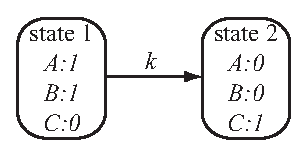
\epsfig{file=figures/two-state.eps, scale=0.7}
\caption{\label{fig:two-state} The Markov Process induced by the reaction 
$A+B \xrightharpoon[\text{}]{\text{$k$}} C$ .
}
\end{figure}




\section{Simple Examples}


In general, the rate matrix for a Markov process is constructed as
follows. The $Q_{i,i}$ matrix is the negative sum of the rates leaving
state $i$. The $Q{i,j}$ matrix, for $i \neq j$, is the rate from state
$j$ to state $i$. Furthermore, when $Q$ is small (say fewer than $1000
\times 1000$), the probability vector $p$ can be solved for explicitly:
%%
$$
p(t) = e^{Qt} p(0) .
$$
%%
All of the statistics, such as the mean copy number and variance of
particular species, can be obtained from $p(t)$.  Several examples are now
given.

\begin{example}
  Suppose we look at the same reaction, $A+B
  \xrightharpoon[\text{}]{\text{$k$}} C$, as above, except where there
  are initially $4$ $A$ molecules and $3$ $B$ molecules. This leads to
  a system with four states, which correspond to the number of $C$
  molecules in the system, either $0$, $1$, $2$, or $3$. Call
  these states $0$ though $3$. The rate at which the system progresses
  from state $0$ to state $1$ has to do with the probability that some
  $A$ reacts with some $B$ to produce a $C$. There are $4 \times 3 =
  12$ possible such pairs, and so probability of transition from state
  $0$ to $1$ in time $[0,dt)$ is $12k$. The rest of the transitions
  are similar. The entire Markov process is shown in
  Figure~\ref{fig:abc}.

\begin{figure}
\centering
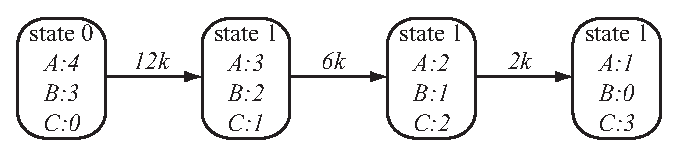
\epsfig{file=figures/abc.eps, scale=0.7}
\caption{\label{fig:abc} The Markov Process induced by the
  reaction $A+B \xrightharpoon[\text{}]{\text{$k$}} C$ where initially
  there are $4$ $A$s, $3$ $B$s, and $0$ $C$s.  }
\end{figure}

\begin{figure}
\centering
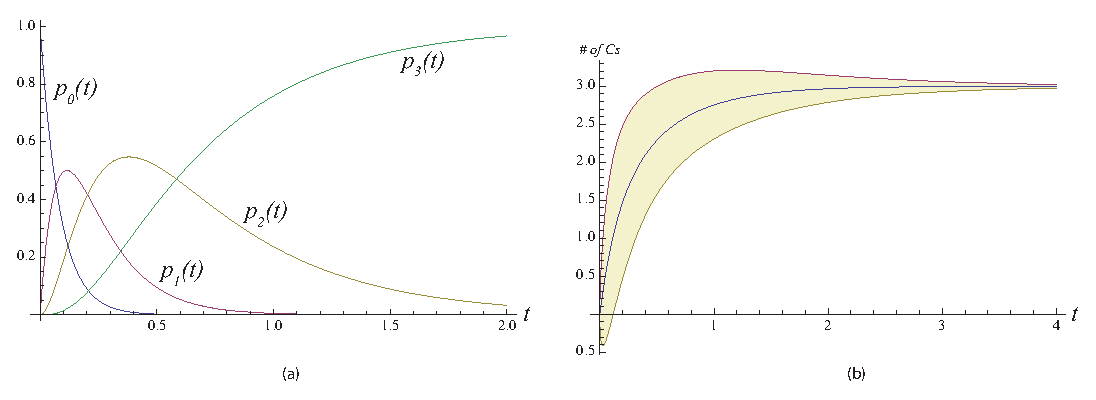
\epsfig{file=figures/abc-stats.eps, scale=0.7}
\caption{\label{fig:abc-stats} (a) The probabilities of being in one
  of the states of the Markov Process in Figure~\ref{fig:abc} versus
  time (for $k=1$). (b) The mean number of $C$s and the one-standard
  window. }
\end{figure}

Kolmogorov's equation for this system, $\dot p = Q p$, is
%
$$
\left ( \begin{array}{c}
\dot p_0 \\
\dot p_1 \\
\dot p_2 \\
\dot p_3 
\end{array}
\right ) = \left (
\begin{array}{cccc}
-12 k & 0 & 0 & 0 \\
12 k & 6k & 0 & 0 \\
0 & -6k & -2k & 0 \\
0 & 0 & 2 k & 0 
\end{array}
\right  )\left ( \begin{array}{c}
p_0 \\
p_1 \\
p_2 \\
p_3 
\end{array}
\right ) .
$$
%
This equation can be solved\footnotemark \ to obtain:
%
\begin{eqnarray*}
p_0(t) & = & e^{-12 t} \\
p_1(t) & = & 2 e^{-12 t} \left ( e^{6kt} - 1 \right ) \\
p_2(t) & = & 2\frac{3}{5} e^{-12 t} \left ( e^{2kt} - 1 \right)^2 \left ( 2 + 4 e^{2kt} + 6 e^{4kt} + 3 e^{6kt}\right ) \\
p_2(t) & = & 2\frac{1}{5} e^{-12 t} \left ( e^{2kt} - 1 \right)^3 \left ( 1 + 3 e^{2kt} + 6 e^{4kt} + 5 e^{6kt}\right )  .
\end{eqnarray*}
%
From the above expressions, we can obtain the mean number of $C$ molecules
%
$$
\ev C = \sum_i i p_i = 3 - \frac{1}{5} e^{-12 t} - e^{-6 t} - \frac{9}{5} e^{-2 t}
$$
%
and the second moment
$$
\ev{C^2} = \sum_i i^2 p_i = 9 - e^{-12 t} + e^{-6 t} - 9 e^{-2 t} .
$$
Figure~\ref{fig:abc-stats}(a) shows the probabilities versus time. The
initial state contains no $C$s. The probabilit of those states decays
exponentially. The probability of the intermediate states increases
and then decreases, and finally all the probability is absorbed in the
final state. Figure~\ref{fig:abc-stats}(b) shows the mean number of $C$s
and the one standard deviation window (calculated from $\ev{C}$ and
$\ev{C^2}$) for the reaction. 
\enx
\end{example}


\footnotetext{To find the solution to $\dot x = A x$ where $A$ is a
  matrix, we use the result that $x(t) = e^{At} x(0)$ where $e^A = I +
  A + A^2/2! + A^3/3! + ...$. The matrix $e^{At}$ can be found in
  MATLAB using the {\tt expm} function or in {\em Mathematica} using
  the {\tt MatrixExp} function.}


% A <-> B
\begin{example} \label{ex:ab}
Consider the reaction 
%
$$
A \xrightleftharpoons[k_2]{k_1} B
$$
and suppose we start with two $A$s and two $B$s for a total of $4$
molecules and five states. Then we arrive at a five state Markov
process with
%
$$
Q = \left ( \begin{array}{ccccc}
-4 k_2 & k_1 & 0 & 0 & 0 \\
4 k_2 & -k_1-3k_2 & 2 k_1 & 0 & 0 \\
0 & 3 k_2 & -2 k_1 -2 k_2 & 3 k_1 & 0 \\
0 & 0 & 2 k_2 & -3 k_1 - k_2 & 4 k_1 \\
0 & 0 & 0 & k_2 & -4 k_1
\end{array} \right ) 
$$
where index $i$ corresponds to the state in which there are $i$ $A$
molecules and $4-i$ $B$ molecules. 

If we start with some arbitrary number of molecules $n$, the
above matrix could only be written schematically, and it would be
difficult to obtain the moments of $A$ and $B$, as we did in the
previous example, in terms of $n$. In the next section, we describe a
method that sometimes workds for dealing with this kind of
problem. \enx
\end{example}

In general, if a system has a mass vector, so that new molecular mass
is not created, then resulting Markov process has a (possibly very
many) finite number of states. If a system can produce molecules from
nowhere, even if they are degraded at some rate, then there can in
principle be any number of such molecules in the system, resulting in
an infinite number of states. The next two examples describe
conservative and a non-conservative systems.

\begin{figure}
\centering
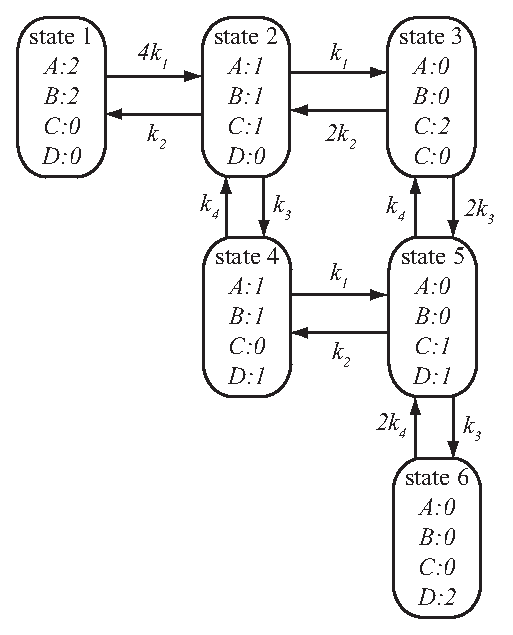
\epsfig{file=figures/cons.eps, scale=0.8}
\caption{\label{fig:cons} The Markov process for the chemical reaction in Example~\ref{ex:cons}.
}
\end{figure}

\begin{example} \label{ex:cons}
The system 
%
\begin{eqnarray*}
A + B & \rreact{k_1}{k_2}  & C  \\
C & \rreact{k_3}{k_4} D 
\end{eqnarray*}
is conservative (show this). The Markov process it produces, given
initially two $A$s, two $B$s and no $C$s or $D$s is shown in
Figure~\ref{fig:cons} and the resulting rate matrix is 
%%
$$
Q = \left (
\begin{array}{cccccc}
-4 k_1 & k_2 & 0 & 0 & 0 & 0 \\
4k_1 & -k_1-k_2 -k_3 & 2 k_2 & k_4 & 0 & 0 \\
0 & k_1 & -2k_2-2k_3 & 0 & 0 & 0 \\
0 & k_3 & 0 & -k_1 - k_4 & k_2 & 0 \\
0 & 0 & 2 k_3 & k_1 & -k_2-k_3 & 2 k_4 \\
0 & 0 & 0 & 0 & k_3 & -2k_4 
\end{array}
\right )
$$ \enx
\end{example}



% 0 -> X -> 0
\begin{example} \label{ex:stoch-gene-master} 
Consider the open-loop expression and degradation of a gene $X$ according to
%
$$
\varnothing \react{k_1} X \react{k_2} \varnothing .
$$
Probalistically speaking, this system can produce any number of $X$
molecules. The result is a Markov process with an infinite number of
states $0$, $1$, $2$, ... describing the number of $X$ molecules in
the system. We can describe the rate of change of the probabilities of
these states by the inifinite set of differential equations
%
$$
\begin{array}{rlllllll}
\dot p_0 & = & -k_1 p_0 & + k_2 p_1           &                  &                  &           \\
\dot p_1 & = &  \;\;\; k_1 p_0 & - (k_1+k_2) k_2 p_1 & + 2 k_2 p_2      &                  &           \\
\dot p_2 & = &          & \;\;\;k_1 p_1             & - (k_1+2k_2) p_2 & 3 k_2 p_3        &           \\
\dot p_3 & = &          &                     & \;\;\; k_1 p_2          & - (k_1+3k_2) p_3 & 4 k_2 p_3 \\
         & \vdots &     &                     &                  &                  & 
\end{array}
$$
Some useful information can be gained from this set of equations. For
example, the steady state distribution can be found as follows. First,
set the above equations to zero. The first equation gives
%
$$
p_1^* = \frac{k_1}{k_2} p_0^*.
$$
%
Adding the first two equations gives
%
$$
0 = -k_1 p_1^* + 2 k_2 p_2 *
$$
%
from which we obtain
%
$$
p_2^* = \frac{k_1}{2k_2}p_1^* = \frac{k_1^2}{2k_2^2} p_0^* .
$$
%
In general, adding the first $n$ equations gives
%%
$$
p_n^* = \frac{\alpha^n}{n!} p_0^*
$$
where $\alpha = k_1 / k_2$. Thus, we have all of the probabilities at
steady state in terms of $p_0^*$, which we can determine by noting
that the sum of the probabilities should be~1. That is
%
$$
\sum_{n=0}^\infty p_n^* = \sum_{n=0}^\infty \frac{\alpha^n}{n!} p_0^* 
                        = 1 \Leftrightarrow \sum_{n=0}^\infty \frac{\alpha^n}{n!} = \frac{1}{p_0^*} .
$$
%
The infinite sum evaluates to $e^{\alpha}$ so that $p_0^* = e^{-\alpha}$ and in general,
%
$$
p_n^* = \frac{\alpha^n}{n!}e^{-\alpha}.
$$
From this result, we can obtain, for example, the mean and second
moment:
%%
$$
\ev X^* = \sum n p_n^* = \alpha  = \frac{k_1}{k_2} 
$$
%%
and
$$
\ev{X^2}^* = \sum n^2 p_n^* = \alpha + \alpha^2 .
$$
%
Using the fact that the standard deviation of $X$ is $\sqrt{ \ev{X^2}
  - \ev X^2}$ be get that the simple result that the standard
deviation in $X$ is $\sqrt \alpha = \sqrt{k_1/k_2}$.
%
%%
\enx
\end{example}

\section{Moment Dynamics}

When there are an arbitrary number of molecules present in the system,
explicity enumerating the Markov process doesn't really work. For
example, consider Example~\ref{ex:ab} in which we enumerated the
states for $A \rreact{}{} B$ for two molecules. We might like to know
the statistics of how many molecules of $A$ we have at equilibrium,
independent of the initial number of $A$s and $B$s. The other problem
is that the system may have an infinite number of states, in which
case it may be difficult to reason about what is going on, although we
were successul with the example $\varnothing \react{} X \react{}
\varnothing$.

Another way to proceed is to use the {\em extended generator} to
produce the moment dynamics of a random variable of interest. Suppose
we have a reaction network with state space $S$ and having transitions
$1,2,3, ..., r$ with rates $k_1$, $k_2$, ..., $'k_r$. Define a {\em
  test function} over the state space by $\psi$. For example, $\psi$
might take a state $s$ and return the number of $A$ molecules in that
state.  The rate of change of the expected value of
$\psi$ follows the simple formula
%
\begin{equation} \label{eqn:moment}
\frac{d}{dt} \ev \psi = \ev{L \psi}
\end{equation}
%
where $L$ is the extended generator, defined by
%
\begin{equation} \label{eqn:generator}
L \psi = \sum_{i=1}^r ( \psi(s') - \psi(s) ) k_i .
\end{equation}
%
In the equation for $L$, we sum over all reactions $i$ the rate
$k_i$ times the difference of the value of $\psi$ after the reaction
and the valueof $\psi$ before the reaction. We can put any polynomial
we like into the equation for $\psi$, such as $A$ or $A^2$ to get the
rate of change of the first and second moments.

\begin{example}\label{ex:ab-moment}
Again, consider the reaction
%
$$
A \rreact{k_1}{k_2} B
$$
that we first encountered in example $\ref{ex:ab}$. This system has
two reactions, the rate of the first is $k_1 A$ and the rate of the
second is $k_2 B$. In general, the generator is
%
$$
L \psi = \left ( \psi \vvec{A-1}{B+1} - \psi \vvec{A}{B} \right ) k_1 A
       + \left ( \psi \vvec{A+1}{B+-1} - \psi \vvec{A}{B} \right ) k_2 B .
$$
%
We can use the generator to determine the rate of change of the
expected number of $A$ and $B$ molecules. We have
%
\begin{eqnarray*}
L A & = & ( A - 1 - A ) k_1 A + ( A + 1 - A ) k_2 B = -k_1 A + k_2 B \\
L B & = & ( B + 1 - B ) k_1 A + ( B - 1 - B ) k_2 B = k_1 A - k_2 B
\end{eqnarray*}
%
Therefore, using Equation~\eref{eqn:moment} we have
%
\begin{eqnarray*}
\frac{d}{dt} \ev A & = &  - k_1 \ev A + k_2 \ev B \\
\frac{d}{dt} \ev B & = &  k_1 \ev A - k_2 \ev B .
\end{eqnarray*}
%
We can also determine the second moment dynamics. These are given by
%
\begin{eqnarray*}
L A^2 & = & ( ( A-1 )^2 - A^2 ) k_1 A + ( ( A+1 )^2 - A^2 ) k_2 B \\
      & = & ( -2A + 1 ) k_1 A + ( 2A + 1 ) k_2 B \\
      & = & k_1 A - 2 k_1 A^2 + k_2 B + 2 k_2 A B .
\end{eqnarray*}
Notice that if we put the above into the Equation~\eref{eqn:moment},
we would get the rate of change of $\ev{A^2}$ in terms of the moments
$\ev A$, $\ev B$, and $\ev{A^2}$ (which we already know), but also
$\ev{AB}$. We could expand this as well, but note that $A+B=n$ is
constant. So instead, we get
%
\begin{eqnarray*}
\frac{d}{dt} \ev{A^2} & = & k_1 \ev A - 2 k_1 \ev{A^2} + k_2 n - k_2 \ev{A}
        + 2 k_2 n \ev A - 2 k_2 \ev{A^2} \\
 & = & k_2 n + ( k_1 - k_2 + 2 k_2 n ) \ev A - 2 ( k_2+k_1 ) \ev{A^2} . 
\end{eqnarray*}
Note: we could also have eliminated the equation for $\ev B$ and the
result would be the rates of change of $\ev A$ and $\ev{A^2}$ in terms
of $\ev A$ and $\ev{A^2}$ .
%
\enx
\end{example}

\begin{example}\label{ex:gene-moment}
Consider again the gene expression example
%
$$
\varnothing \react{k_1} X \react{k_2} \varnothing .
$$
%
We have for the first moment
%
$$
L X = k_1 - k_2 X
$$
%
so that 
%
$$
\ev X = k_1 - k_2 \ev X
$$
%
and $\ev X^* = \frac{k_1}{k_2}$. For the second moment
%
\begin{eqnarray*}
L X^2 & = & ( (X+1)^2 - X^2 ) k_1 + ( (X-1)^2 - X^2 ) k_2 X \\
      & = & ( 2X + 1 ) k_1 + ( -2X+1 ) k_2 X \\
      & = & k_1 + ( 2k_1+k_2 ) X -2 k_2 X^2
\end{eqnarray*}
so that
%
$$
\ev{X^2} = k_1 + (k_1+k_2) \ev X - k_2 \ev{X^2} .
$$
%
At equilibrium, we have
%
\begin{eqnarray*}
\ev{X^2} & = & \frac{k_1 + (2k_1+k_2)\frac{k_1}{k_2}}{2k_2} \\
         & = & \frac{k_1}{k_2} + \frac{k_1^2}{k_2^2}
\end{eqnarray*}
which is the same result as in Example~\ref{ex:stoch-gene-master}. 
%
\enx
\end{example}

The extended generator is a powerful tool for accessing the statistics
of a stochastic chemical reaction, but it does have limitations, which
we now describe. Suppose a system has molecules $A$, $B$, $C$. The
moments of interest are usually the first moments $\ev A$, $\ev B$,
$\ev C$ and the second moments $\ev{A^2}$, $\ev{AB}$, $\ev{AC}$,
$\ev{B^2}$, $\ev{BC}$, etc. There are higher order moments too, such
as $\ev{A^2BC^3}$, but one typically is not concerned with these. One
promising looking result is that the dynamics of each moment are
linear in the rest of the moments. That is, if we stack all the
moments in an infinite dimensional vector $\mu$, then $\dot \mu = A
\mu + B$ describes the rate of change of all the moments, where $A$ is
an infinite dimensional matrix and $B$ is an infinite dimensional
vector.

However, it may be that lower order moments depend on high order
ones. This is not the case in Examples~\ref{ex:ab-moment}
and~\ref{ex:gene-moment} where the rate of change of the first moments
depend on only the first moments; the rate of change of the second
moments depend on the rate of change of the first and second; and so
on. We call this property {\em moment closure}: The rates of change of
all moments depend only on themselves and lower order moments. This
property, when present, makes the moment equations easy to solve.  A
general result, that the above two examples share, is as follows.

\begin{theorem}
  The moment dynamics of a system of reactions in which each reaction
  is no more than unimolecular (involving one or fewer reactants) are closed.
\end{theorem}

For bimolecular reactions, which includes many systems of interest,
the moments are typically not closed, as the following example shows.

\begin{example}
Considera again the reaction
%
$$
A + B \react{k} C .
$$
%
Note that if there are initially $n_A$ As, $n_B$ Bs and zero $C$s, we
have the conservation laws $A = n_A - C$ and $B = n_B - C$. Therefore,
we can simply look at the moments of $C$. We have
%
$$
L C^n = \left ( (C+1)^n - C^n \right ) A B k = \left ( (C+1)^n - C^n \right ) ( n_A - C ) ( n_B - C ) k, 
$$
%
which is an $n+1$ order polynomial. Thus $\ev{C^n}$ depends on
$\ev{C^{n+1}}$ and the moments are not closed.
%
\enx
\end{example}


\section{Approximate Methods}

% approximating the state space

A discussion of the finite state projection algorithm goes here.

\section{Simulation}

Analytical methods for solving stochasti processes are hard to come
by, and are not always easy to analyze. A common recourse is to 

Simulating stochastic processes can be difficult. A naive approach,
and one that is really the best you can do for arbitrary stochasti
processes, is to choose what will happen in the next $delta$ seconds,
where $\delta>0$ is a small number. For example, if there are two
reactions that can occur, one with rate $k_1$ and one with rate $k_2$,
then one would roll a three sided die with weights
%
$$
p_1 = \delta k_1, \;\; p_2 = \delta k_2, \;\; p_3 = 1 - \delta(k_1+k_2) . 
$$
%
If the die comes up with option 1 or 2, the state is updated. If the
die comes up with option three, the state is not update. Then the time
is updated by $\delta$ seconds and the process continues. 

There are several problems with this approach. First, it is
approximate: The trajectories obtained in this manner are not exactly
drawn from the correct distribution, although they sampling becomes
more correct as $\delta \rightarrow 0$. Second, if $\delta$ is small,
then the only thing that happens in most steps is that the time is
updated. This is because the probability that something happens in the
next $\delta$ seconds approaches zero as $\delta$ approaches zero! So
the more accurate the simulation, the longer it takes to simulate.

% the hard way: k dt

Continuous time Markov processes are actually much easier to
simulate. The observation that one can ``exactly'' simulate the Markov
process arising from a stochastic chemical reaction is due to
Gillespie \cite{gillespie}. The algorithm is called the {\em
  Stochastic Simulation Algorithm} or SSA, but is oftern referred to
as the {\em Gillespie Algorithm}.

To explain how it works, consider a Markov process with states
$1,2,3,...$. Suppose the current state is $i$ at time $0$. We would
like to know the joint probability $P[t,j]$ that the next transition
is from $i$ to $j$ and occurs in time $[t,t+dt]$. We can use the rate
$k_{i,j}$, which is the probability that an $i$ to $j$ transition
occurs in the next $dt$ seconds, to get
%
\begin{equation} \label{eqn:Ptj}
P[t,j] = P[T>t] k_{i,j} dt
\end{equation}
%
where $P[T>t]$ is the probability that the transition does not occur
in time $[0,t]$.

We can derive a similar expression for $P[T>t+dt]$. First note that 
%
$$
\left ( 1 - \sum_{j=1^N} k_{i,j} \right ) dt = ( 1 - K_i )
$$
%
is equivalent to the probability that no transition occurs in the next
$dt$ seconds. Here, we have defined $K_i = \sum_{j=1}^N k_{i,j}$ to be
the total rate out of state $i$. Thus,
%
$$
P[T>t+dt] = P[T>t] ( 1 - K_i ) dt . 
$$
Rearranging gives
%
$$
\frac{P[T>t+dt] - P[T>t]}{dt} = - P[T>t] K_i.
$$
%
The left hand side of this is $\frac{d}{dt}P[T>t]$. Solving this
differential equation for $P[T>t]$ and substituting into
Equation~\eref{eqn:Ptj} gives
%
\begin{equation}\label{eqn:ssa-pdf}
P[t,j] = k_{i,j} e^{-K_i t} .
\end{equation}
%
We can now determine how to choose the next state and the next reaction time.

\paragraph{Next Reaction:} Integrating Equation~\eref{eqn:ssa-pdf}
over all time gives the probability that the next reaction is $j$, no
matter what time it occurs.
%
\begin{equation}\label{eqn:next-reaction}
p_{i,j} = \int_0^\infty  k_{i,j} e^{-K_i t} dt = \frac{k_{i,j}}{K_i} .
\end{equation}
%
Thus, to choose the next reaction, we roll an $N$ sided die, with
weights $p_{i,j}$ for $j=1,N$.

\paragraph{Reaction Time:} To choose the time, we sum over all
reactions to get that the proabilility densitiy function for the next
reaction time is
%
$$
\sum_{j=1}^N k_{i,j} e^{-K_i t} = K_i e^{-K_i t}. 
$$
%
The cumulative distribution function corresponding to this function is
%
$$
\int_0^t K_i e^{-K_i t\tau} d \tau = 1 - e^{-K_i t} = r \in [0,1],
$$
which relates $t$ distributed according to the Poisson distribution
$K_i e^{-K_i t}$ and $r$ distributed uniformly in $[0,1]$. Since
computers can pick uniform random numbers easily, we solve for $t$ to
get
%
\begin{equation}\label{eqn:next-time}
t = \frac{1}{K_i} \ln \frac{1}{1-r} .
\end{equation}
%
Therefore, to choose the next time in a simulation, we choose $r$
uniformly in $[0,1]$ and then compute the time according to the above.

\paragraph{The SSA:} Now, using the above results, we describe the
Stochastic Simulation Algorithm. 
\begin{enumerate}
\item[1.] Choose an initial condition $v$ equal to some vector of the copy
  numbers of the species in the reaction network.
\item[2.] Set $t=0$.
\item[3.] For each reaction $\rho$ applicable in $v$, determine the rate $k_v$. 
\item[4.] Choose the next reaction via Equation~\ref{eqn:next-reaction}.
\item[5.] Choose the $\Delta t$ via Equation~\ref{eqn:next-time} and set
  $t$ to $t+\Delta t$. 
\item[6.] Goto 3.
\end{enumerate}

In practice, one typically sets a maximum time and a maximum number of
steps to force a termination condition. Also, a single trajectory is
usually not sufficient to characterize the behavior, so multiple
trajectories are sampled (say thousands) and combined to obtain sample
averages. 

\begin{figure}
  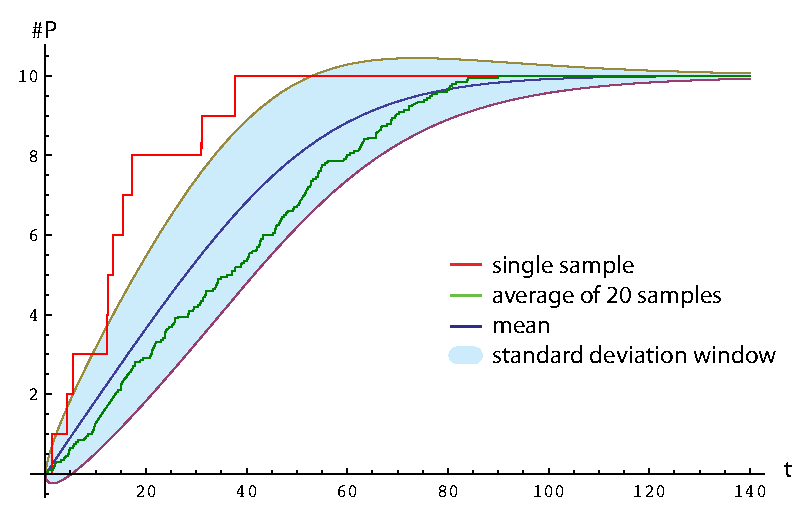
\epsfig{file=figures/stochastic-mich-ment.eps, scale=0.7}
  \caption{\label{fig:mm-stoch} The Michaelis-Menton system from
    Example~\ref{ex:mm-stoch}. Shown are a sample trajectory (red), 20
    samples averaged together (blue) and the mean and standard
    deviation window computed from the Kolmogorov Equation. }
\end{figure}

\begin{example} \label{ex:mm-stoch}
Consider the reaction network
%
$$
E + S \rreact{k_1}{k_2} ES \react{k_3} E + P 
$$
where $k_1=1$, $k_2=0.5$ and $k_3=0.1$. Starting in a state $v_1 =
(E,S,ES,P) = (2,10,0,0)$ at time $t=0$, the only reaction applicable
is the first. Thus the probability that the next state is $(1,9,1,0)$
is $1$. The reaction has rate $20 k_1 = 20$. The time the reaction
occurs is distributed according to the p.d.f. $20 e^{-20t}$. From the
state $(1,9,1,0)$ there are three possible reactions with rates
%
$$
9, \; 0.5, \; \mathrm{and} \; 0.9 .
$$
Thus, the probabilities of each of these reactions are
%%
$$
\frac{9}{10.4}, \; \frac{0.5}{10.4}, \; \mathrm{and} \; \frac{0.9}{10.4}
$$
%
and the p.d.f. of when the reaction occurs is distributed according to
$10.4 e^{-10.4 t}$. Figure~\ref{fig:mm-stoch} shows a typical sample
trajectory along with the average of 20 samples, and the mean and
variance computed from the Kolmogorov Equation in which all 30 states
are enumerated. 
%
\end{example}



\section{Computing with Molecules}

One of the central questions of synthetic biology is whether and how
computations can be carried out with molecular systems. Many
researchers have tried to answer this question and computations have
been done with oligos \cite{adleman-science94} and DNA self-assembly
\cite{winfree-assembly} for example. Furthermore, many models of
molecular computation have been proposed
\cite{rozenberg-dna-computing}. Here, we examn one such model, which
is an implementation of regiester machines \cite{minsky-rms} by
stochastic chemical reaction networks \cite{soloviechik-rm}.

A {\em register machine} is a kind of abstract computational
machine. It is equivalent in expressibility to the Turning Machine
model, and thus any algorithm can in principle be implemented as a
register machine. Register machines consist a finite set of states
$S_0$, $S_1$, ..., $S_n$ and a set of registers $R_0$, $R_1$, ...,
$R_m$. Register machine transitions have of two types. The first is an
increment:
%
$$
\mathrm{inc}(i,r,j)
$$
%
which means {\em if the state is $i$, then increase register $r$ and
  go to state $j$}. The second is a decrement:
%
$$
\mathrm{dec}(i,r,j,k)
$$
%
which means {\em if the state is $i$ and register $r$ is greater than
  zero, then decrease register $r$ and go to state $j$; otherwise go
  to state $k$.}. 

Register machines can be written as diagrams, as in
Figure~\ref{fig:rm-mult}, which describes a register machine that can
multiply. The increment transitions are simply arrows from $i$ to $j$
with the register $r$ being incremented shown by the arrow. For
example, the arrow from state $2$ to $3$ labeled $\uparrow 2$
describes the command $\mathrm{inc}(2,2,3)$. The decrement transitions
are similar, except that a dashed arrow describes what state to go to
if the register being decremented is zero.

\begin{figure}
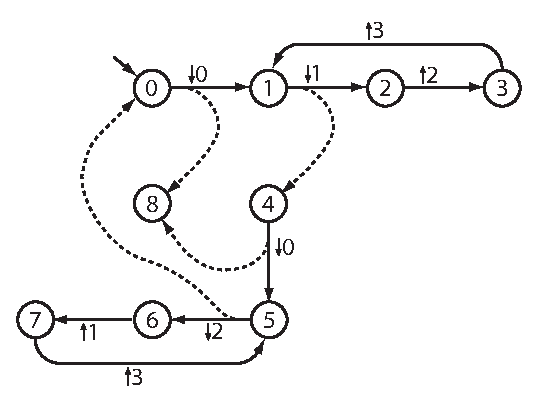
\epsfig{file=figures/rm-mult.eps, scale=0.9}
\caption{\label{fig:rm-mult} A register machine that multiplies the
  initial contents of registers $0$ and $1$. Register $3$ holds the
  final value and register $2$ is swap space.}
\end{figure}

To implement a register machine with stochastic chemical reactions, we
do the following. First, introduce a new chemical species $S_i$ for
each sate. We will require that at any given time, the total number of
state molecules of any kind is $1$. Also, we introduce new chemical
species $R_i$ for every register. The number of $R_i$ molecules in the
system at a given time corresponds to the value of that register at
that time. Next, for each increment transition $\mathrm{inc}(i,r,j)$
in the system we introduce the reaction
%
$$
S_i \react{k} S_j + M_r. 
$$
%
Finally, for each decrement transition $\mathrm{dec}(i,r,j,k)$ we
introduce the two reactions
%
$$
S_i + M_r \react{k} S_j
$$
and
$$
S_i \react{\varepsilon} S_k .
$$
%
The first decrement reaction describes the interaction of an $S_i$
molecule with an $M_r$ molecule. This reaction has rate $M_r k$ so
that if there are no $M_r$ molecules, the reaction rate is zero. The
second reaction is the ``else'' part of the decrement rule. If there
are no $M_r$ molecules, then eventually this section reaction should
occur. However, there is some small probability
%
$$
\frac{\varepsilon}{\varepsilon+M_r k}
$$
%
that the second decrement reaction might occur even if there are $M_r$
molecules around. Thus, we would like $\epsilon$ to be small. On the
other hand, when it is not an error to take the second decrement
reaction, we sould like the rate to be large. This tradeoff is
fundamental to this formulation: {\em accurate computation takes
  longer}.

\begin{figure}
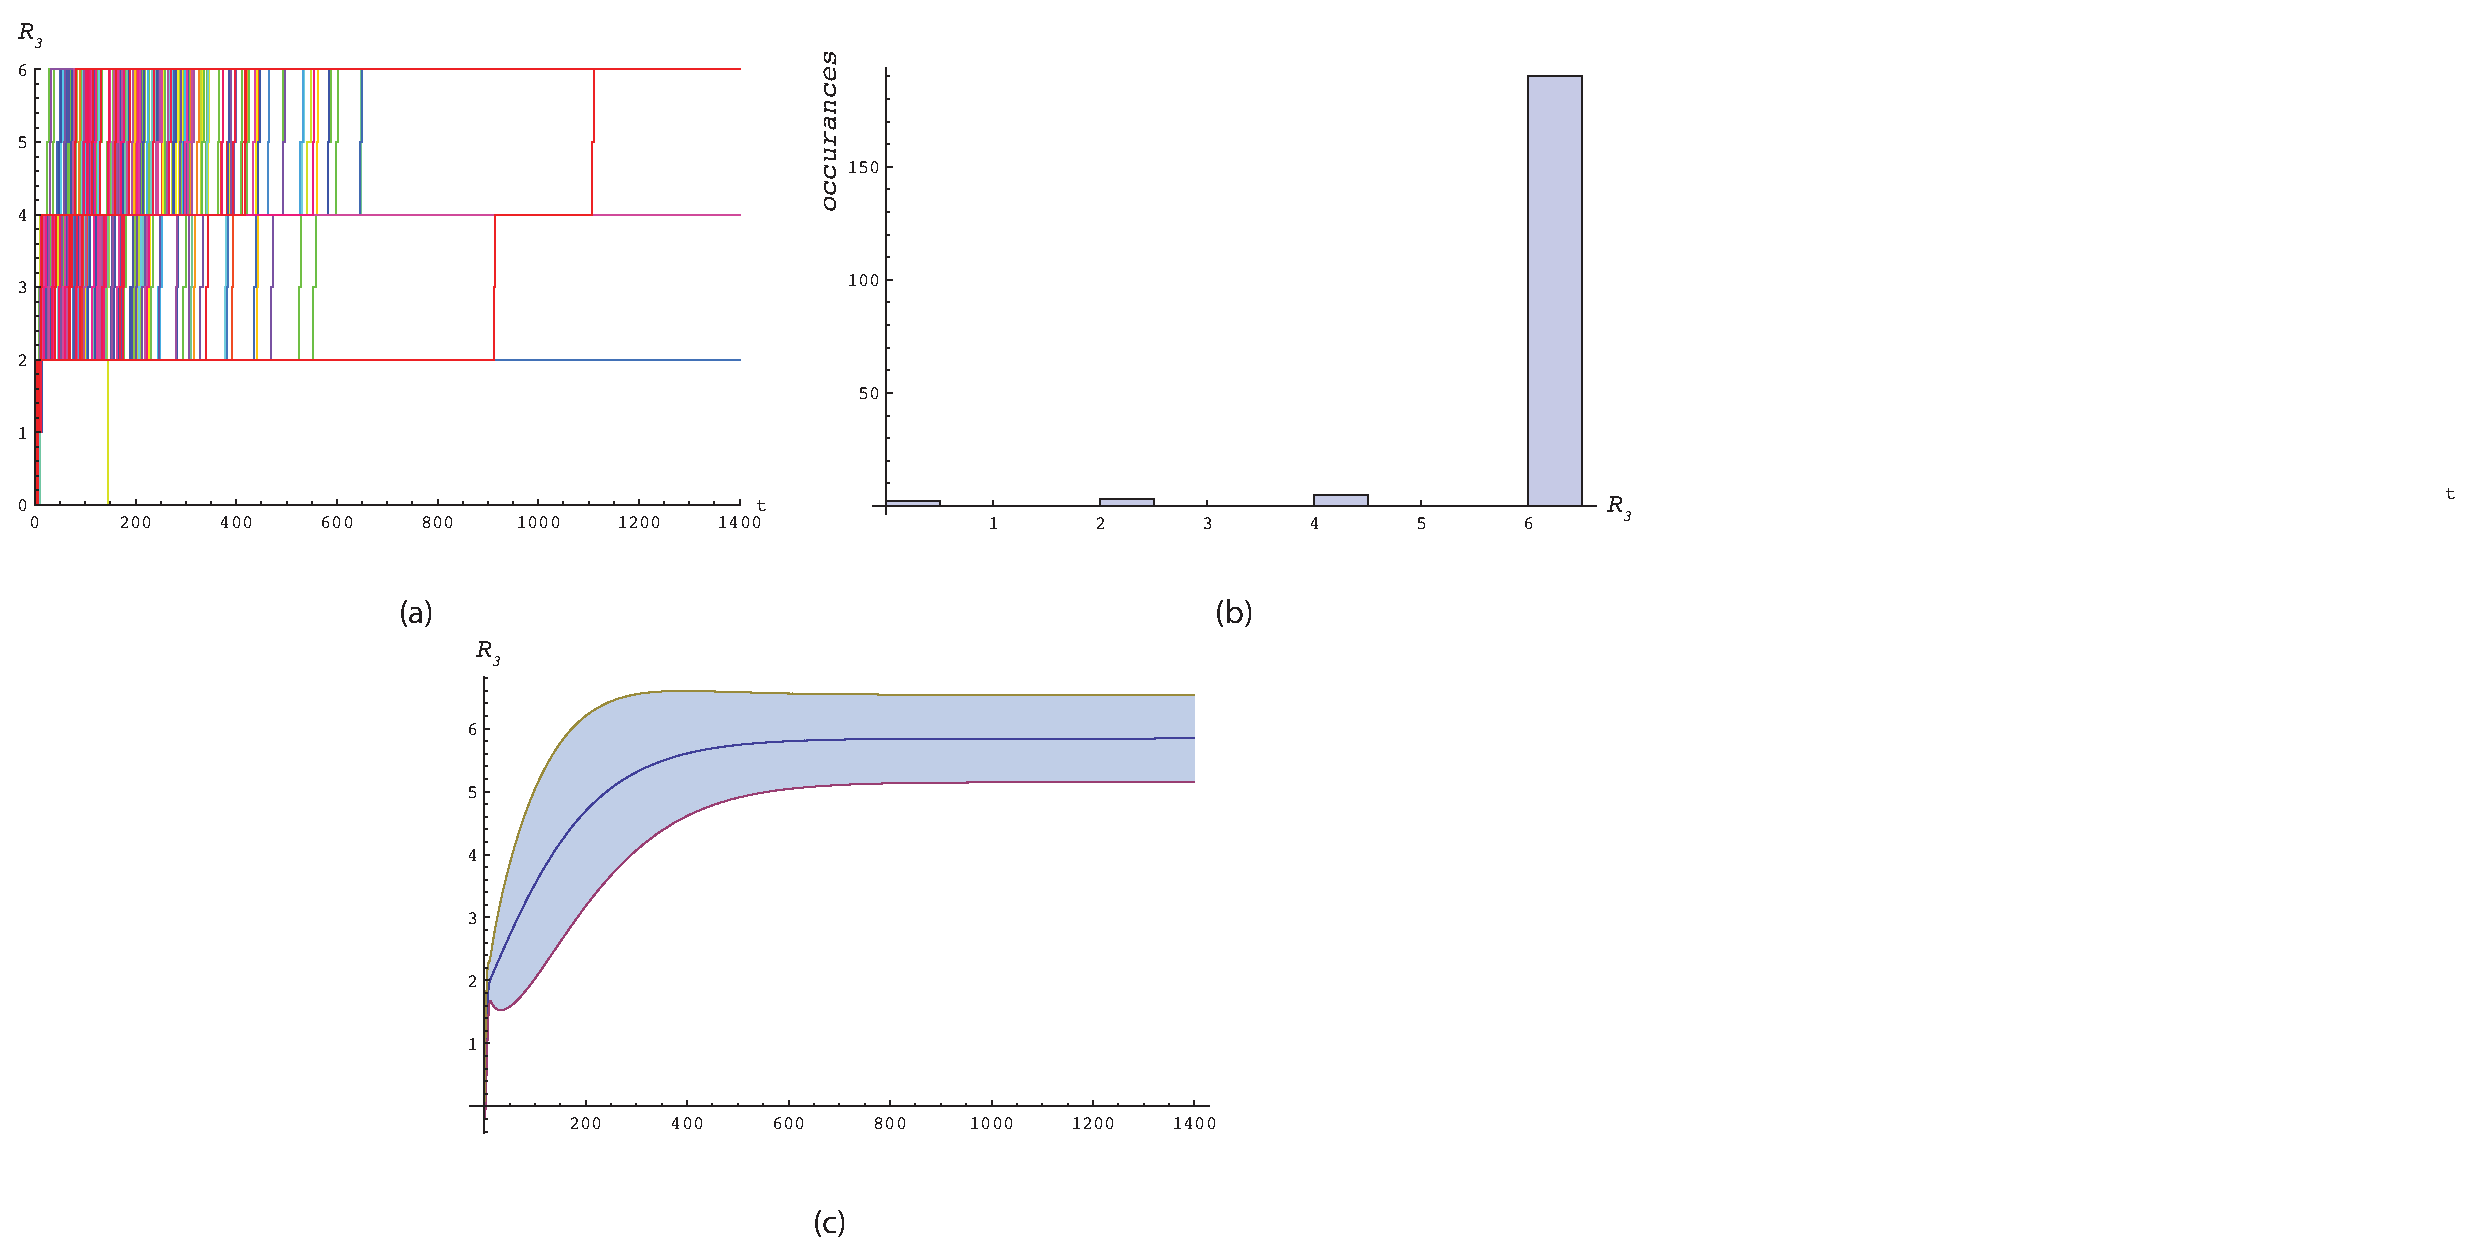
\epsfig{file=figures/rm-behavior.eps, scale=0.45}
\caption{\label{fig:rm-mult-data} (a) Several trajectories of the
  chemical implementation of the multiplication register machine
  computing $2 \times 3$. (b) The histogram of the computed
  results. (c) The mean and standard deviation behavior computed from
  the Kolmogorov equation.}
\end{figure}


\begin{example}
  The register machine\footnotemark in Figure~\ref{fig:rm-mult}
  multiplies the contents of registers $R_0$ and $R_1$ and puts the
  result in register $R_3$. This can be implemented with twelve
  reactions: two each for the decrement reactions and one each for the
  increment reactions. Figures~\ref{fig:rm-mult-data}(a) and~(b) shows
  the resulting behavior when computing $2 \times 3 = 6$ with $k=1$
  and $\epsilon=0.01$. Stochastic simulations show the system can end
  up with the result $0$, $2$, $4$ and $6$ with the most likely answer
  being the correct one. Figure~\ref{fig:rm-mult-data}(c) shows the
  exact solution. Using the methods in this chapter, the entire state
  space (of the Markov process) was enumerated to yield 78 states and
  a $78 \times 78$ dimensional rate matrix. Shown are the average
  number of $R_3$ molecules and the standard deviation window. \enx
\end{example}

\footnotetext{The author thanks Kevin Oishi for finding a way to
  multiply with register machines.}




\section{Problems}

\setcounter{exercount}{0} 

\begin{exercise}\label{ex:exponential}
  Show that if $G(t+\tau) = G(t)G(\tau)$ is analytical and integrable,
  then $G(t) = e^{-\alpha t}$ for some $\alpha > 0$.
\end{exercise}

\begin{exercise}
Consider the reaction network
%
\begin{eqnarray*}
A & \react{k_1} & B + C \\
C + D & \rreact{k_2}{k_3} & E 
\end{eqnarray*}
%
starting with two $A$s and two $D$s and no $B$s, $C$s or $E$s. (a)
Enumerate the states and draw the Markov process the results from this
system. (b) Determine the rate matrix. (c) Find the probabilities of
being in each state as a function of time by finding $e^{Qt}p(0)$. (d)
Find the mean and variance for the number of $E$s as a function of
time and plot the mean and the one standard deviation window versus
time (as in Figure~\ref{fig:abc-stats}(c)) assuming all the rates are
unity. Note: To simiplfy things, you may set $k_1=1$, $k_2=1$, and
$k_3=1$. Also, if you use MATLAB or Mathematica to compute the
solution, you do not need to show the output if it is large, just show
the code.
\end{exercise}

\begin{exercise}
  Show that if a system of reactions admits a mass vector, then the
  Markov process describing its stocahstic behavior has a finite
  number of states. Give an example of a non-conservative system that
  still produces a finite number of states.
\end{exercise}

\begin{exercise}
  For the gene production and degradation system described in
  Examples~\ref{ex:stoch-gene-master} and~\ref{ex:stoch-gene-moments},
  determine the number $n$ such that the probability of there being
  more than $n$ molecules of $X$ at steady state is less than 1\%. 
\end{exercise}

\begin{exercise} \label{exer:ab-probs}
  Determine the time varying probabilities of being in the various
  states of Example~\ref{ex:ab}. Plot the probabilities versus time
  for the case when both rates are~1 and we start with no $B$
  molecules.
\end{exercise}

\begin{exercise}
  Verify that the moment equations for $\ev A$ and $\ev{A^2}$ obtained
  in Example~\ref{ex:ab-moment} match those obtained using the
  solutions from Exercise~\ref{exer:ab-probs}. 
\end{exercise}



\begin{exercise}
Consider the system
%
$$
\varnothing \react{k_1} X \react{k_2} Y \react{k_3} \varnothing .
$$
Using equations~\eref{eqn:moment} and~\ref{eqn:generator}, determine
equations for $\ev X$, $\ev Y$, $\ev{X^2}$, and $\ev{Y^2}$ versus
time. Determine the steady state values for the means and standard
deviations. Starting from no molecules, plot the expected number of
$X$ and $Y$ molecules and standard deviation windows (as in
Figure~\ref{fig:abc-stats}(c)) assuming the rates are all unity.
%
\end{exercise}



\begin{exercise}
\item Consider the network
%
$$
EA+S \rreact{k_1}{k_{-1}} EAS \react{k_2} EA + P
$$
$$
E+A \rreact{k_3}{k_{-3}} EA
$$
\noindent
with rates

\hspace{0.5in}\begin{tabular}{ll}
$k_1$    & 9.3 $s^{-1}$ \\
$k_{-1}$ & 1.2 $s^{-1}$ \\
$k_2$    & 0.5 $s^{-1}$ \\
$k_3$    & 5.0 $s^{-1}$ \\
$k_{-3}$ & 1.5 $s^{-1}$. 
\end{tabular}
\begin{enumerate}
\item[a)] Suppose the initial number of $E$, $A$ and $S$ molecules is 2, 1
  and 4 respectively and the initial number of the remaining molecule
  types is 0. Draw the Markov process that results.
\item[b)] Plot the mean and standard deviation window for the number
  of $P$ molecules as a function of time, as in
  Figure~\ref{fig:mm-stoch}. You should obtain these either by solving
  the Kolmogorov Equation via $e^{Qt}$ or simply simulating the
  differential equations. You should find $\ev P$ and $\ev {P^2}$ as
  functions of time, and use these to find the standard deviation as a
  function of time.
\item[c)] Simulate the system 20 times using the stochastic simulation
  Make a plot of one of the trajectories and of the average of all the
  trajectories showing the number of $P$ molecules, as in
  Figure~\ref{fig:mm-stoch}.
\end{enumerate}
\end{exercise}

\begin{exercise}
Consider the system
%
$$
\varnothing \react{k_1} X \react{k_2} \varnothing,
$$
which produces an infinite dimensional Markov process. Kolmogorov's
equation for this system has an infinite dimensional $Q$ matrix. In
this exercise, you will approximate this matrix wirth a series of
finite matrices. Define $Q(n)$ to be the rate matrix for the
following approximation to the above system 
%
$$
0 \rreact{k_1}{k_2} 1 \rreact{k_1}{2k_2} 2 \rreact{k_1}{3k_2} ... \rreact{k_1}{nk_2} n .
$$
%
Consider the case when $k_1=5$ and $k_2=1$ and there are initially no
$X$ molecules. Using $\dot p = e^{Q(n)t} p(0)$, plot the mean number
of $X$ molecules (plus standard deviation windows) versus time for
$n=5, \; 10, \; 20, \; 30, \;\mathrm{and}\; 40$. How could this idea
be used to approximate the behavior any reaction network, with a
finite number of states or not?
%
\end{exercise}



\begin{exercise}
  Write down the chemical reactions for the multiplication register
  machine shown in Figure~\ref{fig:rm-mult}. 
\end{exercise}

\begin{exercise}
  What is the probability that the chemical implementation of the
  multiplication register machine computes $1 \times 1$ incorrectly
  (in terms of $k$ and $\varepsilon$?). 
\end{exercise}

\begin{exercise} \label{ex:rm-even}
  Find a register machine that determines whether the initial value of
  of register $R_0$ is even or odd. If it is even, the machine should
  terminate with a $0$ in register $R_1$. Otherwise, it should
  terminate with a $1$ in register $R_1$. 
\end{exercise}

\begin{exercise}
  Find the stochastic chemical reaction implementation of the register
  machine you found in Exercise~$\ref{ex:rm-even}$. Using Gillespie's
  algorithm, simulate the reaction network 100 times for $5$ initial
  $R_0$ molecules and plot the results. Do it again for $6$ initial
  $R_0$ molecules. Find Kolmogorov's equations for $5$ initial $R_0$
  molecules and plot the mean and standard deviation windows the
  expected number of $R_1$ molecules. Use $k=1$ and $\varepsilon=0.1$.
\end{exercise}

\begin{exercise}
  Propose an idea for how the chemical implementation of register
  machines could be implemented inside cells. Where else would errors
  come from in your implementation? Give an example of a computation
  that would be useful in a synthetic biology setting.
\end{exercise}

\begin{exercise}
  (Extra Credit) Find a register machine that computes $n!$ for $n
  \geq 0$. Simulate the chemical implementation of it using
  Gillespie's algorithm. 
\end{exercise}

